\documentclass[a4paper,12pt]{article}

\usepackage{url}
\usepackage{amsmath}
\usepackage{amssymb}
\usepackage{epsfig}
\usepackage{mathtools}
\usepackage{graphics}
\usepackage{fancyhdr}
\usepackage{cite}
\usepackage{algorithm}
\usepackage[noend]{algpseudocode}
\usepackage{tikz}

\usepackage{color}
\usepackage{colortbl}
\definecolor{LightGray}{gray}{0.9}

\graphicspath{{pictures/}}

\title{Report for assignment 2 in the course DD2438 at KTH}
\author{\hspace*{-0.5cm}
GROUP10\\
\begin{tabular}{cccc}
Arash Safari & Ermias Gebremeskel \\
%BIRTHDATE1 & BIRTHDATE2 \\
asafari@kth.se & ermiasg@kth.se \\
%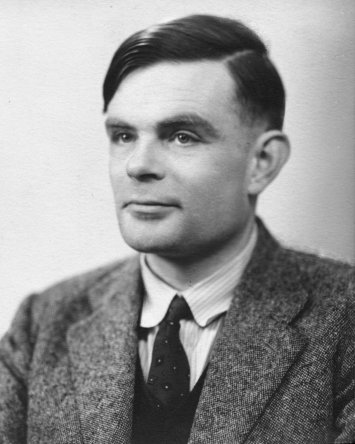
\includegraphics[width=0.13\linewidth]{Alan_Turing_photo} & 
%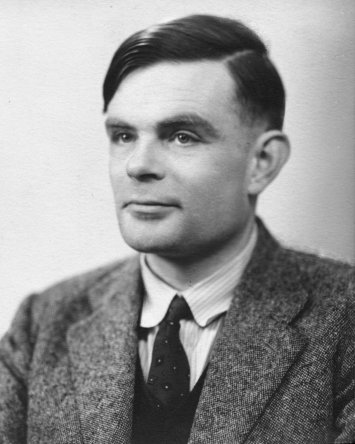
\includegraphics[width=0.13\linewidth]{Alan_Turing_photo}
\end{tabular}} 
\date{}

\pagestyle{fancy}
\setlength{\headheight}{15pt}
\fancyhf{}
\lhead{DD2438 agent16} % DO NOT REMOVE!!!!
\rhead{Arash Safari, Ermias Gebremeskel} %% UPDATE WITH YOUR NAMES
\begin{document}

\maketitle
\thispagestyle{fancy}

\begin{abstract}
This paper will discuss formation keeping, collusion avoidance, and vehicle routing problems in the context of autonomous systems with different motion models. This is done by researching and implementing different approaches to the three problems in a simulation environment and analysing the results. The final implementation includes formation keeping with point and car motion models, a force field based collusion avoidance, and vehicle rout finding that tries to minimizing time using Simulated Annealing and finds the actual trajectory to be followed by a model using Rapidly exploring Random Tree (RRT).  
 
\end{abstract}



\clearpage

%%%%%%%%%%%%%%%%%%%%%%%%%%%%%%%%%%%%%%%%%%%%%%%%%%%%%%%%%%%%%
%%%%%%%%%%%%%%%%%%%%%%%%%%%%%%%%%%%%%%%%%%%%%%%%%%%%%%%%%%%%%
\section{Introduction}
\label{sec:intro}

Manoeuvring in formation is a desired characteristic for autonomous robots with applications ranging from  synthesizing a space-based interferometer to covering a grid\cite{945797} or moving large objects using multiple robots. There are two main control architectures or strategies for formation keeping: leader follower\cite{350940} \cite{637948} and virtual structure\cite{960341}. In leader follower one robot will be designated as the leader and the other robots will pursue the leaders motion with an offset that represent the formation, and the stability of the tracking error is controlled via feedback control like proportional–integral–derivative controller (PID) or a fuzzy controller\cite{bazoula2008formation}. On the other hand in virtual structure the formation is seen as a structure with place holders for each robot, where robots are striving to keep their place in the virtual structure. Two scenarios of formation keeping are discussed in this paper: the first one is where robots have global knowledge  of their environment. Where as in the second scenario robots only have knowledge of the environment around them given by a visibility radius. The leader following approach to formation keeping is simple to implement and reliable in the global knowledge scenario where there is only one leader, but when it comes to the local knowledge where robots follow leaders closest to them the chain of feedback controls can create a butterfly effect that can magnify the tracking error down the chain making the formation unstable.  

When manoeuvring in an environment where multiple autonomous robots are present collusions are imminent. The problem of finding a collusion free path for robots manoeuvring among static and dynamic obstacles is there for of great importance. The straight forward and easiest way to collusion avoidance is a force-based virtual spring where obstacles have force fields around them that repels robots that came near them. The main disadvantage of this strategy is that the force fields do not take in to consideration the velocity of the robot and the presence of other obstacles. A more reliable approach to collusion avoidance are velocity obstacles(VO)\cite{wilkie2009generalized}\cite{van2008reciprocal}. In Velocity obstacles every agent calculates reachable velocities that will not lead to collusion by considering the velocities of near by agents, and intersecting the velocity obstacle of all agents with in a given radius. Even though this is a reliable approach to collusion avoidance it requires knowledge of every agent's velocity. The final problem discussed in this paper is the vehicle routing problem. The "Vehicle Routing Problem"(VRP), is a combinatorial optimization problem similar to the "Travelling Salesman Problem"(TSP) concerned with the optimal design of a path to be used by a fleet of robots to complete a set of tasks. In this paper the basic VRP with no capacity constraint is considered.      
 

\subsection{Contribution} 
 This project is done as an assignment in an introductory course in robotics and does not consist of any real contribution to the field of robotics. Most of the algorithms used in this report are simplifications of already well known and established algorithms. 
The report will however, hopefully be useful to any novice in the field seeking an insight into formation keeping, collusion avoidance, and vehicle routing problems.

\subsection{Outline}
In the Section~\ref{sec:relwork},we will describe the related work that we consulted during the execution of the project. The project itself consists of solving three different problems, which are described together with the attempted solutions in the Section~\ref{sec:method}. The experimental setup, as well as details about the experiments themselves can be found in Section~\ref{sec:exps}. And finally, a short summary of the report is given in the Section~\ref{sec:summary}.
 

%%%%%%%%%%%%%%%%%%%%%%%%%%%%%%%%%%%%%%%%%%%%%%%%%%%%%%%%%%%%%
%%%%%%%%%%%%%%%%%%%%%%%%%%%%%%%%%%%%%%%%%%%%%%%%%%%%%%%%%%%%%

\section{Related work}
\label{sec:relwork}
In this Section, the theoretical back ground needed to understand this paper and a short description of few related works that we found useful before and during the implementation of our solutions are discussed.
\subsection{Formation Keeping}
\label{sec:fk}
Formation keeping is a desired characteristic for autonomous robots with many applications. Depending on the application different control architectures can be used.          

\subsubsection{Leader-Follower Formation}
\label{sec:lf}
The leader follower architecture is particularly well-suited in situations where agents have global knowledge i.e only one leader, but can get unstable when there are more than one leaders. This instability comes from followers trying to correct their tracking error which in-turn introduces a slightly bigger tracking error to their followers.
A formation in the leader follower architecture is represented by a relative distance as shown in figure 1 and a bearing angle between the leader and the follower\cite{bazoula2008formation}. 

\begin{figure}
\centering
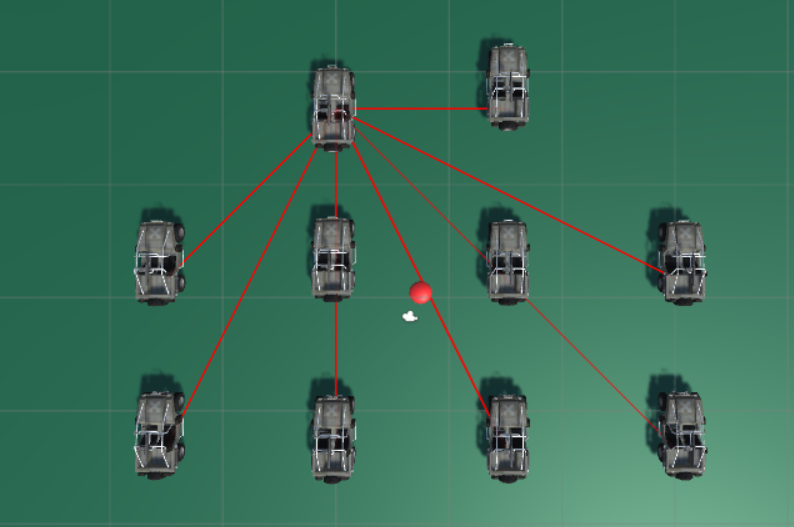
\includegraphics[width=0.8\linewidth]{Leader-Follower}
\caption{A leader with the relative position of the followers shown in red lines.}
\label{fig:Leader-Follower}
\end{figure}  

In order for the follower mobile robot to pursue the leader they need to make slight adjustments to their speed and bearing angles. This adjustments depend on the tracking error of the agents and use the error as a feedback for the controller. A simple feedback controller can use fuzzy logic. In fuzzy logic unlike boolean logic we can have a degree of truth and falsehood which can be used to decide the control applied to the agent to correct the tracking error.  

\subsubsection{Fuzzy Controller} 
\label{sec:fc}
Fuzzy sets were introduced by Zadeh in 1965 to represent/manipulate data and information possessing non-statistical uncertainties\cite{zadeh1965fuzzy}. The main purpose of the fuzzy controller is to make the follower robot maintain a desired distance and bearing from the leader. The tracking error given by $e(p)=position - desired_p$, $e(v)=e(p)_t - e(p)_{t-1}$, $e(\omega) = angle - desired_a $ and $e(\theta) = e(\omega)_t - e(\omega)_{t-1} $ are decomposed in to fuzzy partitions as described in \cite{bazoula2008formation}. Finally the weighted fuzzy set values are used as feedback to the controller.

\subsection{Velocity Obstacles} 
\label{sec:vo} 
Finding a collusion free path for robots manoeuvring among static and dynamic obstacles is important for any moving robot that does not work in isolation. Velocity obstacle can be used to calculate colliding relative velocities between one or more agents. Figure 2 shows a velocity obstacle for agent A and an obstacle B. We calculate the velocity obstacle between A and B by first enlarging B by the radius of A, and reducing A to a point. The collision cone is then given by the lines starting for $VB$ (velocity of B) relative to the position of A, and are tangent to the enlarged obstacle B'. We can then try to find reachable velocities for A such that $R_{VA}= VA + maxForce*\delta t$ , and is as close to the desired velocity of A but that is outside the collusion cone.

\begin{figure}
\centering
  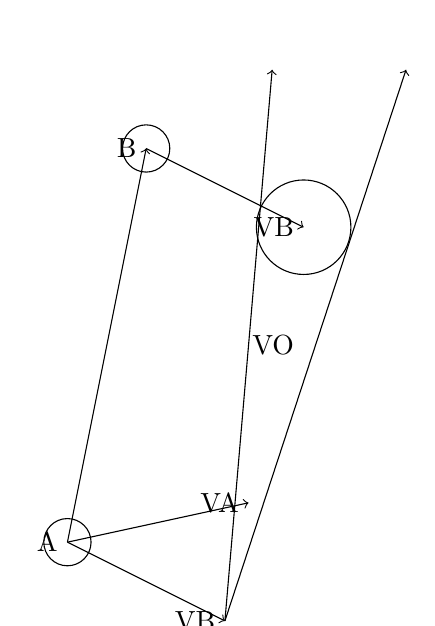
\begin{tikzpicture}[domain=0:4] 
    \draw[thin,color=black](1,5) circle (0.3) node[left] {B};
    \draw[thin,color=black](3,4) circle (0.6);
    \draw [->] (1,5) -- (3,4)node[left] {VB}; 
    \draw[color=black] circle (0.3) node[left] {A};
    \draw[color=black] (3,2.5)circle (0.0) node[left] {VO};
    \draw [->] (0,0) -- (1,5);
    \draw [->] (0,0) -- (2.3,0.5)node[left] {VA};
    \draw [->] (0,0) -- (2,-1)node[left] {VB};
    \draw [->] (2,-1) -- (2.6,6);
    \draw [->] (2,-1) -- (4.3,6);
  \end{tikzpicture}
  \caption{Velocity obstacle calculated by agent A for obstacle B with velocity VB} \label{fig:VO}
\end{figure}
\subsection{Vehicle Routing Problem}
\label{sec:vrp}
The vehicle routing problem is first proposed by Dantzig and Ramser \cite{dantzig1959truck}. There are many variants of this problem, such as the Capacitated VRP, in which the capacity of the vehicles is constrained, vehicle routing problem with Time Windows (VRPTW) where tasks need to be completed in a given time frame, and Mixed Fleet VRP where different type of vehicles with different capacity are used for the problem \cite{golden2008vehicle}. In this paper we will only consider the unconstrained variant of the problem. 

The VRP can be formulated as a graph problem with a directed graph $G(V,E)$, where $V= \{ 0, 1,...,n-1 \}$ is the set of n nodes and E is the set of edges. The nodes represent starting points for the vehicles and the tasks and the edges are roads and their weights represent the cost to get to a node. After creating a graph representation of the problem a tour construction heuristic like nearest Nearest Neighbour, or Greedy can be used to create the initial rout. This can then be optimized using local optimization algorithms like 2-opt, which removes two edges and try to reconnect the resulting two paths in a way that the resulting tour is shorter, this can give some improvement but can get stuck in a local optimum. One way to get out of local optimal solutions is Simulated Annealing\cite{aarts2005simulated}. Simulated Annealing is a randomized local search algorithm that allows for none improving moves to be taken in order to get out of a local optimum. In Simulated Annealing (SA) we set a temperature and a cooling rate and we accept bad moves while the temperature is still high and decrease the acceptance probability with the temperature. This is justified by the high probability of getting an improving move in the beginning but this moves will get scarce after some iterations.   
%%%%%%%%%%%%%%%%%%%%%%%%%%%%%%%%%%%%%%%%%%%%%%%%%%%%%%%%%%%%%
%%%%%%%%%%%%%%%%%%%%%%%%%%%%%%%%%%%%%%%%%%%%%%%%%%%%%%%%%%%%%
\section{Implementation}
\label{sec:method}
The project consisted of three different parts: "Formation keeping", "Vehicle Routing Problem" and "Collision Avoidance". In this section, each of these problems and the attempted solutions will be covered.  
\subsection{Formation keeping}
\label{sec:mmImpl}
In this problem, the agents are placed in predetermined locations and need to enter a formation as fast as possible. Variations of this problem included:
A) Enter formation with global knowledge of the position of other agents.
B) Enter formation with local knowledge of the position of other agents.
C) Enter a moving formation.

Problem A) was solved by simply generating a greedy solution, which then was iteratively improved using an exhaustive search. The improvement process consisted of minimizing the sum of the cubes of the distances each agent had to traverse.
Meaning if vehicle A needed to traverse X meters and vehicle B Y meters, the expression that was minimized was $X^3+Y^3$. This heuristic penalizes the longer distances, and therefore results in a smaller Max distance across all agents. 

Problem B) was solved by trying to get the agents as close to each other as possible so that every agent can see every other agent. This is achieved by following the closest neighbour that is within the visibility radius and to avoid a deadlock leaving one agent with no leader to follow. This ensures every agent will converge to the position of the one agent without a leader. After the agents are close enough to detect each other the same algorithm as problem A is executed.  

Problem C) The moving formation in the case of the global knowledge was implemented with the leader following strategy as mentioned in section \ref{sec:lf} where only the leader have the knowledge of the direction of the formation. On the other hand the local knowledge implementation gives the direction and the formation to every agent ,which will try to come close to each other the same way as Problem B and then choose a position in the formation with first come first served manner. After every position in the formation is is occupied every agent will move to the direction given with the same speed. 

To make sure that every agent is facing the direction of the formation when starting to move, a runway was given for every agent that is long enough to make the agent face the right way.

\subsection{Vehicle Routing Problem}
\label{sec:pf}

The "Vehicle Routing Problem"(VRP), is an NP problem similar to the "Travelling Salesman Problem"(TSP) problem. Unlike the TSP problem, where there is only one traveler traversing every city, we have multiple vehicles that need to divide the cities in between them. 

Our version of the VRP problem had some twists to it.
Firstly, we are minimizing time, and not distance. Secondly the movements our agents can perform are restricted by the agents motion model. 
This means that moving from one point to another is not a simple of traversing an Euclidean distance between the two points. Velocity, acceleration, direction and obstacles all play a major role in the path one would need to take when moving from A to B.

As with most NP problems, creating an algorithm that finds the optimal solution was not plausible. We therefore decided to look for an acceptable solution through the use of "Simulated Annealing".
For this approach, we needed a weighted graph of the map. This was created through the use of "Visibility Graphs" and "A*", using the length of the path created by A* as the weight of the edge. The Simulated Annealing algorithm would then create a greedy solution based on the graph, and make improvements using probabilistic methods.

However, we noticed this solution solved a much too simplified version of the problem at hand.  As explained earlier, the variable being minimized in this problem was time, not distance. Using Euclidean distances as weights in our graphs resulted in finding the shortest path that often could not be followed in a timely manner by a vehicle with restrictive motion models.

Generating accurate weights between each node was not possible due to the weight varying immensely on too many variables such as the ones described earlier. Instead we decided to use the simulated annealing algorithm, not to produce the shortest path, but to produce a large number of short paths. These paths could even be longer than the initial greedy path, as long as they were kept below a set threshold. 

We then would use "Rapidly exploring Random Tree"(RRT), to explore estimate the time it takes for the vehicle to traverse the path, and chose the one that resulted the shortest times.
Of course, this approach results in some additional margins of error, as RRT reacts extremely random. In order to minimize the effect of this additional randomness, we had to have our algorithm run repeatedly over longer periods of time.


\subsection{Collision Avoidance}
\label{sec:pfinding}

The Collision Avoidance problem during this project consisted of detection and avoiding not only obstacles, but also other vehicles with only local knowledge.

Our initial approach to solving the issue was to implement a repulsion mechanism to each agent. Whenever they get too close to an obstacle, or another agent, the agent would calculate the trajectory that would lead to a crash, and move in the exact opposite direction.
This however, lead to some weird behavior when cars in a collision course made symmetrical moves in order to avoid the collision, which then lead to a new collision course. The process would remind a lot of when 2 people try to get out of each other ways at the same time and end up blocking each other more.

The solution to this was to implement a priority order, where cars with higher priority ignore collision risks and the car with the lower priority work harder to try to avoid them. This did not completely work either, as sometimes, both cars need to take action in order for a collision to be avoided. 

A middle ground that worked well in the test cases was to have varying degrees of sensitivity amongst the cars. Where cars with low priority are way more sensitive and try to avoid collisions much earlier than a car with a higher priority, who will only start avoiding a collisions when its imminent.

\subsubsection{Velocity Obstacles}
\label{sec:voI}
The implementation of the velocity obstacle was not completed in time for the deadline of this project and was abandoned.  


%%%%%%%%%%%%%%%%%%%%%%%%%%%%%%%%%%%%%%%%%%%%%%%%%%%%%%%%%%%%%
%%%%%%%%%%%%%%%%%%%%%%%%%%%%%%%%%%%%%%%%%%%%%%%%%%%%%%%%%%%%%
\section{Experimental results}
\label{sec:exps}


\subsection{Experiemntal setup}
The experiments are performed by first creating a virtual map based on the provided specifications. Based on this map, path can be generated for each agent using RRT. These paths are imported by each agent, in the Unity client. Additional settings, such as the physical properties, or behavior patterns such as collision avoidance is set and tuned. At this point the simulation is ran through Unity, and the results are observed and documented. 

\subsection{Experiment}

The experiments consisted of running our algorithms in several different scenarios created specifically to test their efficiency. The exection of these experiments varried depending on the algorithm that was being tested.

In the case of the formation keeping algorithms, we merely had to change some variables(such as the starting points of vehicles and the shape of the formation) to the appropriate values specified for the test, and then let the algorithm take care of the rest. The specifications of the test are listed below:
\begin{itemize}
\item Problem 11a: Global knowledge formation keeping for Dynamic point model with Vmax=100, Amax=1
\item Problem 11b: Local knowledge formation keeping for Dynamic point model with Vmax=100, Amax=1, Sensing radius 20
\item Problem 12a: Moving formation for Differential drive model with Wmax=30 deg/s, Vmax=10
\item Problem 12b: Moving formation for Dynamic car model with L=10, Amax=1, Vmax=10, phimax=45deg
\end{itemize}


For the VRP problem test, the initial path finding algorithm generated 250 randomly generated paths with an euclidean length smaller than that of the original greedy path. These paths were then ran through an RRT algorithm in order to estimate their actual length. Due to the randomness of RRT, the RRT algorithm was ran 100 times for each path, with the fastest result being selected. The specifications of the test are listed below:
\begin{itemize}
\item Problem 13a: Vehicle routing problem for Dynamic point model with Vmax=100, Amax=1
\item Problem 13b: Local knowledge formation keeping for Dynamic point model with Vmax=100, Amax=1, Sensing radius 20
\end{itemize}
, In order to run the experiments, we simply set some variables to the appropriate values of the test, and  to the ones of the motion model. The algorithm would then run repeatedly, remembering its best result. Once a long period of time, usually 20 minutes, passed without a better path being found, the algorithm would stop.
The specifications of the different models were:
\begin{itemize}
\item Problem 11: Kinematic point model with Vmax=10
\item Problem 12: Dynamic point model with 
	\begin{itemize}
	\item 12a: Vmax=20, Amax=40
	\item 12b: Vmax=20, Amax=13
	\item 12c: Vmax=20, Amax=8
	\item 12d: Vmax=100, Amax=20
	\end{itemize}
\item Problem 13: Differential drive model with Vmax=10, Wmax=0.3
\item Problem 14: Kinematic car, Vmax=10, PhiMax=pi/4
	\begin{itemize}
	\item 14a: L=10
	\item 14b: L=30
	\item 14c: L=50
	\end{itemize}
\item Problem 15: Dynamic car, PhiMax=pi/4, Vmax=100, Amax=20
	\begin{itemize}
	\item 15a: L=10
	\item 15b: L=50
	\end{itemize}
\end{itemize}


\subsection{Results}
The strategy described in the previous chapters worked perfectly fine for the simpler models such as the point models, and even the shorter car models.
Thousands of possible paths could be generated within a short period of time.
The best ones of these randomly generated paths were very close to the results of the other groups that did well.
However, when it came to the car models with lenghts of $ >30$, the algorithm could not find any paths at all, even when it was allowed to run for hours.

\begin{table}
    \begin{tabular}{llllllllll}
    ~   & P11a  & P11b       & P12a  & P12b  & P13a    & P13b     & P14a          & P14b  & P15a        \\
    G1  & 16.8  & 26.9(R=30) & 10.3  & 30.2  & ~       & 312      & 27.9          & 11.5  & ~           \\
    G2  & 13.5  & 33.3       & 11.8  & 23.3  & 54.80   & 51.62    & -             & -     & -           \\
    G3  & 17.1  & 34         & 13    & 19    & 48      & 34 (L=1) & 74.2          & 32.4  & 77.9        \\
    G4  & 17.2  & 40.8       & 30    & 28    & ~       & ~        & \\    61\\    & 79    & 170         \\
    G5  & 16    & 36.8       & 45    & ~     & 98.1    & ~        & 77.61         & ~     & 168.72      \\
    G6  & 15.6  & ~          & ~     & 37.7  & > 8 min & 61.4     & 38.5          & 28.5  & ~           \\
    G7  & 16.3  & 21.22      & 11.1  & ~     & 72.02   & ~        & 28.84         & 12.44 & 238.24      \\
    G8  & 23    & 40         & 53    & ~     & 71.83   & 89.92    & 43            & 36.24 & ~           \\
    G9  & 10.89 & 19.03      & 5.76  & 26.00 & 57.56   & 28.90    & 27.45         & 10.04 & 96.6        \\
    G10 & 12.28 & 20.16      & ~     & 25.00 & 68.5    & 53.9     & 49.3          & 22.2  & 163.5       \\
    G11 & 14.4  & 15.5       & 12.6  & 20.3  & 46.8    & 28.3     & 29.3          & 15.3  & 41.6 (min)  \\
    G12 & 18.38 & 30.42      & 37.18 & 30.12 & 72.72   & 50.64    & 61.60         & 20.54 & 193.08      \\
    G13 & 15.38 & 54         & 44    & ~     & 353     & ~        & 63            & 23    & ~           \\
    ~   & ~     & ~          & ~     & ~     & ~       & ~        & ~             & ~     & ~           \\
    \end{tabular}
\end{table}
\pagebreak
%%%%%%%%%%%%%%%%%%%%%%%%%%%%%%%%%%%%%%%%%%%%%%%%%%%%%%%%%%%%%
%%%%%%%%%%%%%%%%%%%%%%%%%%%%%%%%%%%%%%%%%%%%%%%%%%%%%%%%%%%%%
\section{Summary and Conclusions}
\label{sec:summary}
\subsection{Summary}
In summary, we implemented formation keeping with dynamic point and car models and collision avoidance was implemented for dynamic point model and to some extent for the car model. The collision avoidance for the car model need to take in to consideration the maximum steering angle when choosing avoidance velocities. VRP was implemented for both dynamic models.     
\subsection{Conclusions}
The strategy that was adopted in our implementation proved to be successful in comparison with the performance given by other groups as shown in the table above. In the case of the collision avoidance where precision is more desirable than time the force-based implementation we had was inferior to the velocity obstacle implementation done by many groups. 

%%%%%%%%%%%%%%%%%%%%%%%%%%%%%%%%%%%%%%%%%%%%%%%%%%%%%%%%%%%%%
%%%%%%%%%%%%%%%%%%%%%%%%%%%%%%%%%%%%%%%%%%%%%%%%%%%%%%%%%%%%%
\pagebreak
\bibliography{reflist}{}
\bibliographystyle{plain}


\end{document}
